\section{Robot Hardware}
\label{sec:robot_hardware}

\subsection{Torsional Spring Leg}
\label{sec:torsional_spring_leg}

Figure \ref{fig:assembly_CAD} shows the CAD model for the torsional spring leg design, including both knee and hip extension/flexion motor, as well as the hip adduction/abduction motor. The CAD model was created using the CAD software Solidworks. An annotated exploded view of the leg can be seen in figure \ref{fig:CAD_leg_exploded_annotate}, while an annotated exploded view for the hip motor housing can be seen in figure \ref{fig:exploded_motor_housing_hip}. 

Figure \ref{fig:manufacture_only} shows the components that are currently planned to manufacture in inhouse. The axle that will be threaded and screwed directly into the motor shaft, and lead directly into a ball bearing, is emphasized in red. The leg has been designed to make it easily manufacturable in aluminum. Aluminum was chosen as a potential material due to its high strength-to-weight ratio, and the fact that it is easy to machine. Although many easily 3D-printable plastics are generally lighter, they are not as strong as aluminum, in fact aluminum has a much higher weight to yield ratio than 3D printable plastics, and thus, barring complications resulting from manufacture, a leg made in aluminum should be lighter than one made of plastic \cite{Aluminum} \cite{PLA}. 

\begin{figure}[h!]
    \centering
    \begin{subfigure}[b]{0.45\textwidth}
        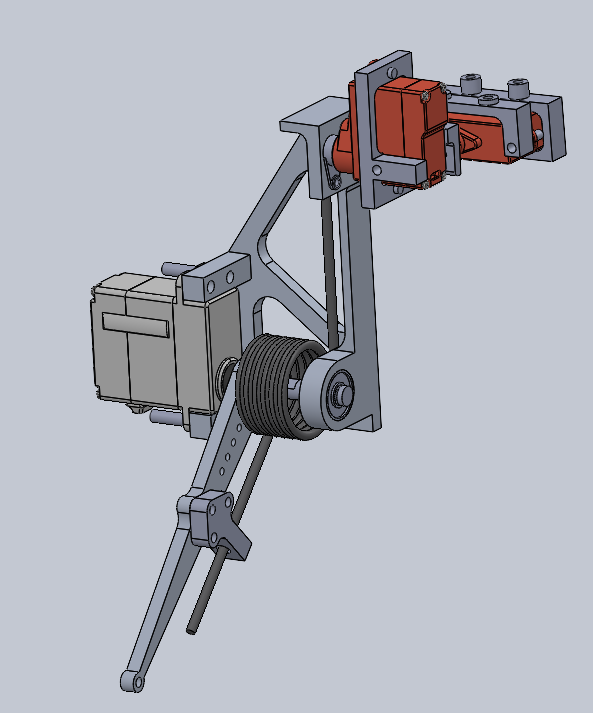
\includegraphics[width=\textwidth]{Images/CAD_leg_inside_bent.png}
        \caption{Notice the bearing holding the knee-joint shaft in place. This is important to reduce the load the motor shaft suffers in directions other than the load direction.}
        \label{fig:image1}
    \end{subfigure}
    \hfill
    \begin{subfigure}[b]{0.45\textwidth}
        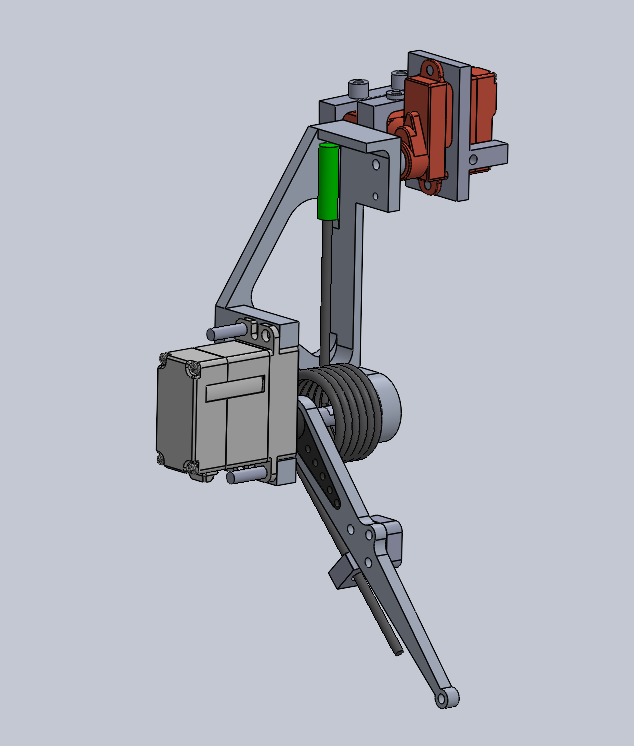
\includegraphics[width=\textwidth]{Images/CAD_leg_outside_bent.png}
        \caption{As can be seen, there is a green plastic (PLA) holster where the spring is in contact with the leg, this is to reduce  friction.}
        \label{fig:image2}
    \end{subfigure}
    \caption{An overview of the leg CAD model with a torsional spring. }
    \label{fig:assembly_CAD}
\end{figure}

\begin{figure}[h!]
    \centering
    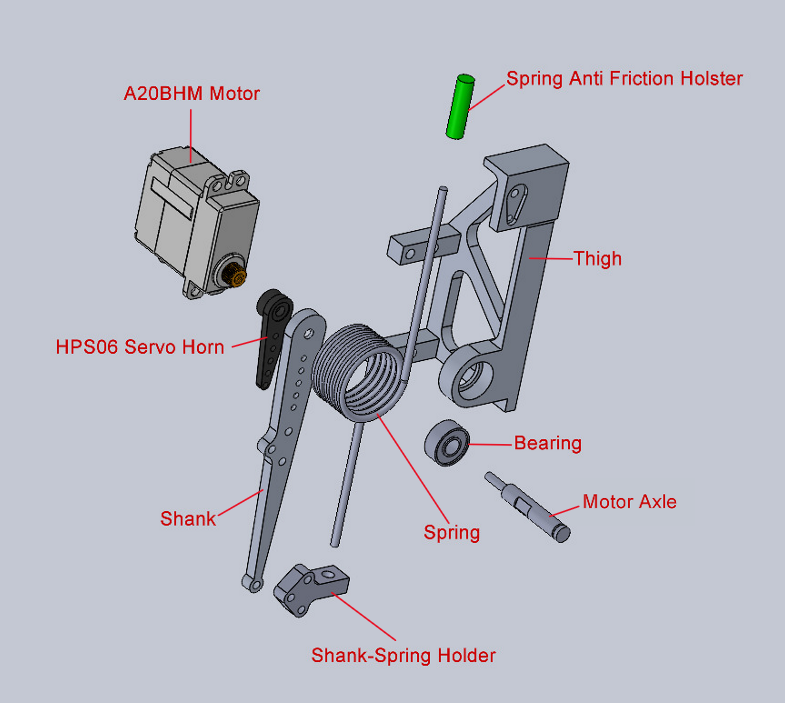
\includegraphics[width=0.6\textwidth]{Images/CAD_leg_exploded_annotate.png}
    \caption{Annotated exploded view of the CAD leg design.}
    \label{fig:CAD_leg_exploded_annotate}
\end{figure}

\begin{figure}[h!]
    \centering
    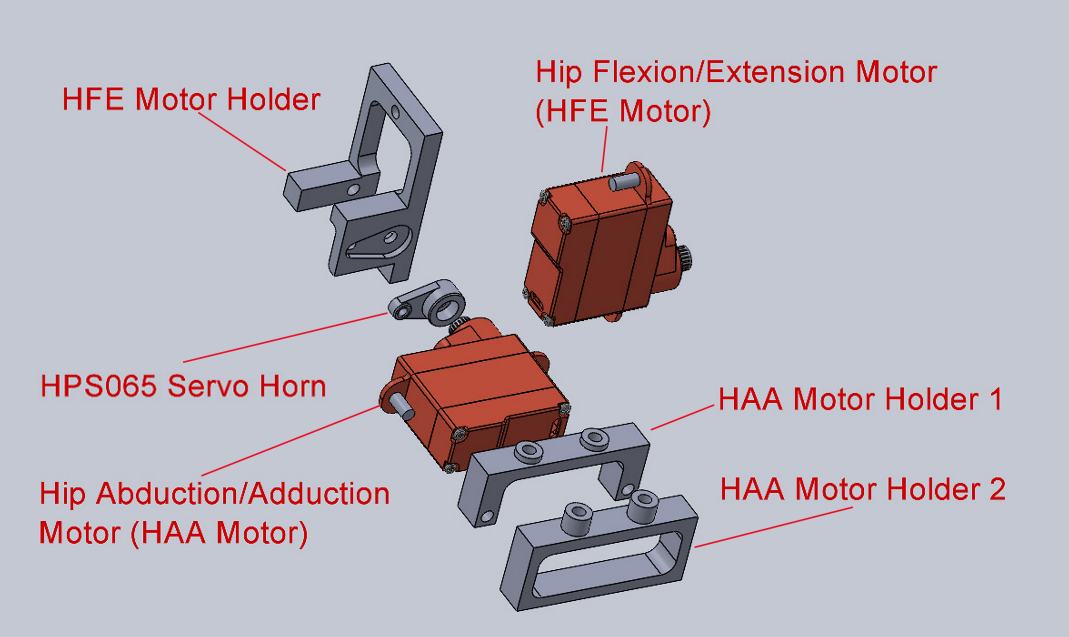
\includegraphics[width=0.6\textwidth]{Images/exploded_motor_holder_hip.png}
    \caption{Exploded view of the motor housings for the hip joint.}
    \label{fig:exploded_motor_housing_hip}
\end{figure}

\begin{figure}[h!]
    \centering
    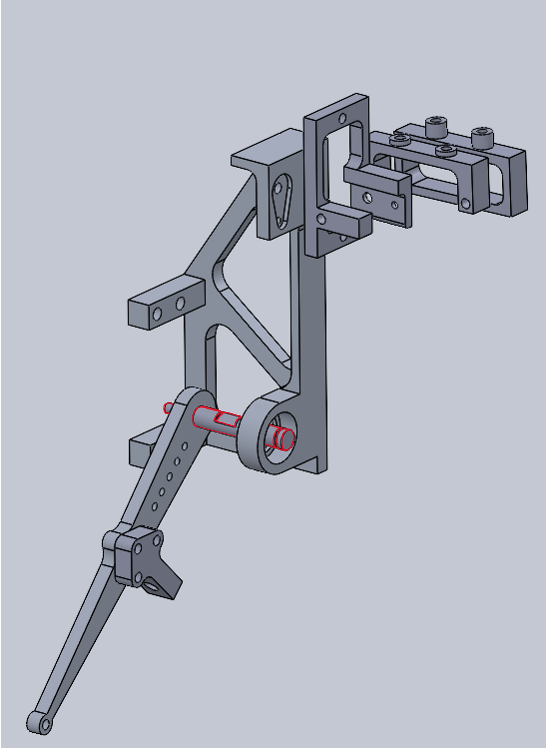
\includegraphics[width=0.6\textwidth]{Images/manufacture_only2.png}
    \caption{An overview of the CAD model of the leg design, but showing only the components that will be manufactured inhouse. Axle that will be threaded and screwed directly into the motor shaft, and lead directly into a ball bearing, is emphasized in red. }
    \label{fig:manufacture_only}
\end{figure}

A 3D printed version of the thigh together with the purchased spring can be seen in figure \ref{fig:printed_leg_and_spring}. While the full leg has not been assembled, initial physical load tests seem to indicate that the thigh is able to withstand the load of the spring. This could indicate that the leg will be 3D printed rather than made in aluminum. The axle that will be screwed into the motor shaft, however, will still be made in aluminum. 

\begin{figure}[h!]
    \centering
    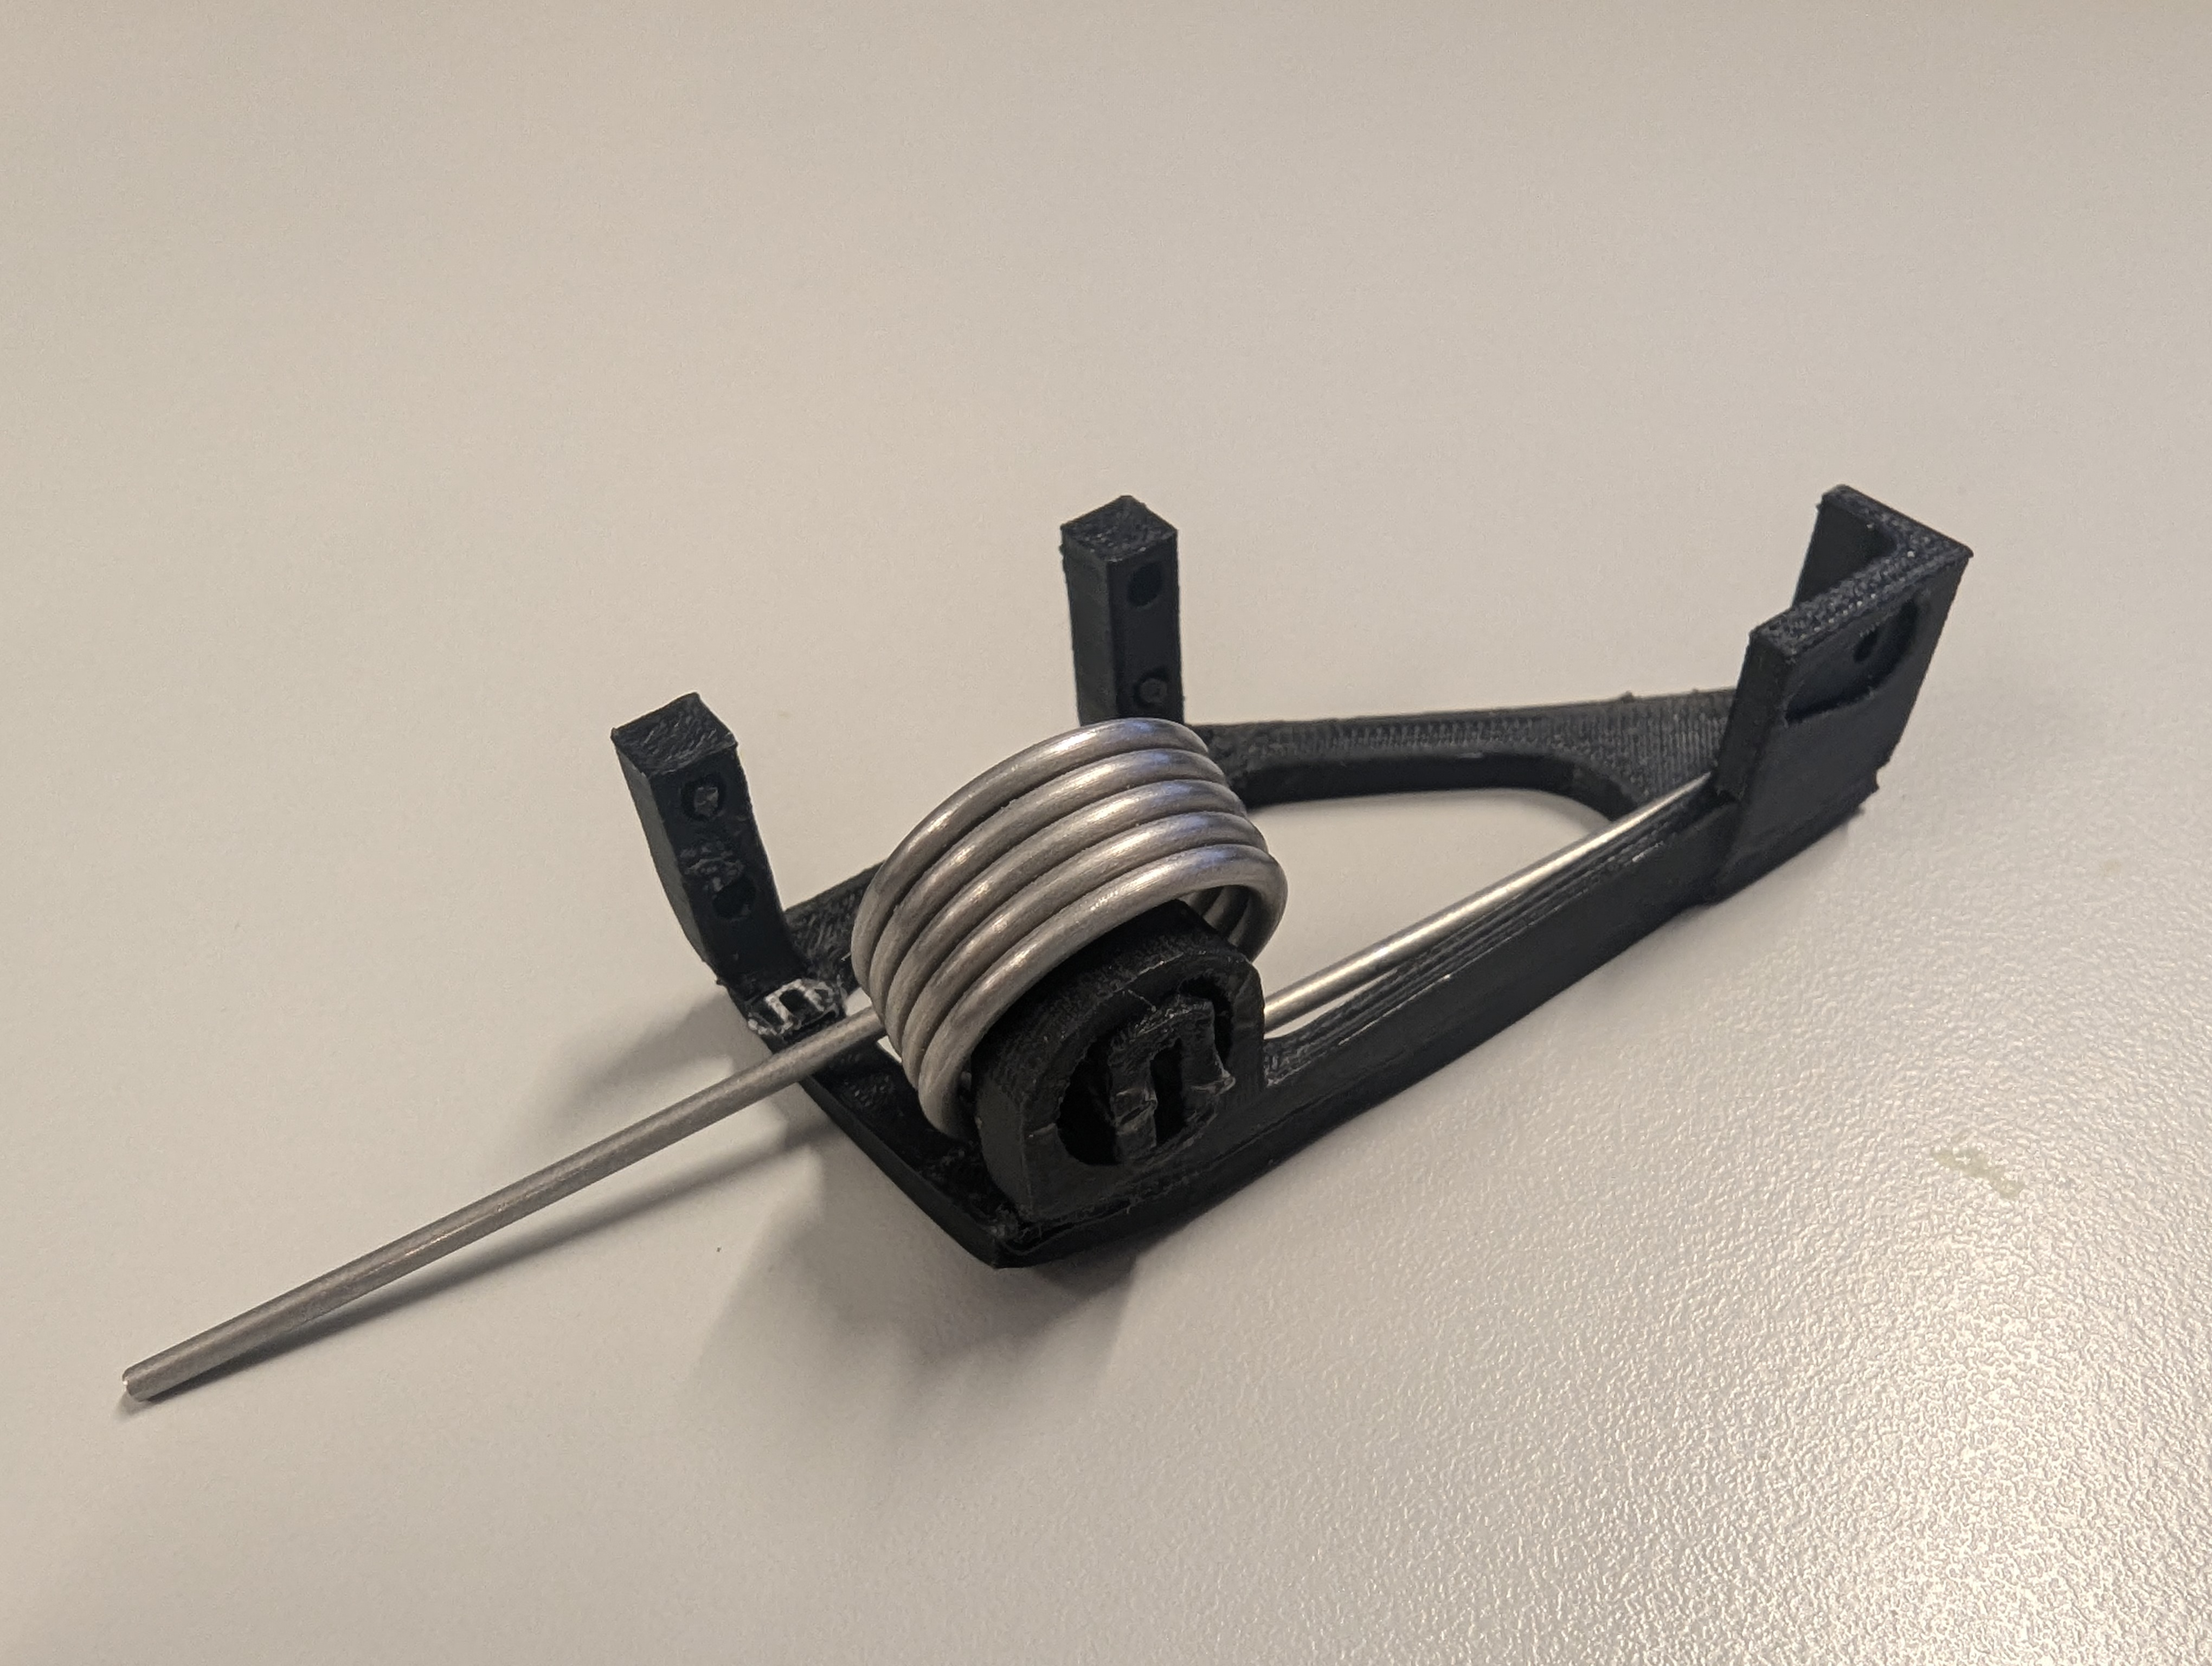
\includegraphics[width=0.6\textwidth]{Images/printed_leg_and_spring.jpg}
    \caption{A 3D printed version of the leg thigh with the torsional spring.}
    \label{fig:printed_leg_and_spring}
\end{figure}

\subsection{Extension Spring Leg design}
\label{sec:extension_spring_design}

The extension spring leg design is shown in figure \ref{fig:extension_spring_CAD}. As can be seen in the figure, the current design is such that the extension spring will collide with the robot shank as the knee angle approaches fully coiled (ie. -180 degrees). Despite efforts, no solutions were found for this problem, and this design direction was therefore abandoned. Among the suggested solutions was moving the shank-end attachment point of the spring inwards towards the body, so the extension spring could lie in parallel next to the shank when the leg is fully coiled. This would however introduce a significant moment arm acting directly on the motor shaft, and this design was therefore abandoned in favor of the torsional spring design.

\begin{figure}[h!]
    \centering
    \begin{subfigure}[b]{0.45\textwidth}
        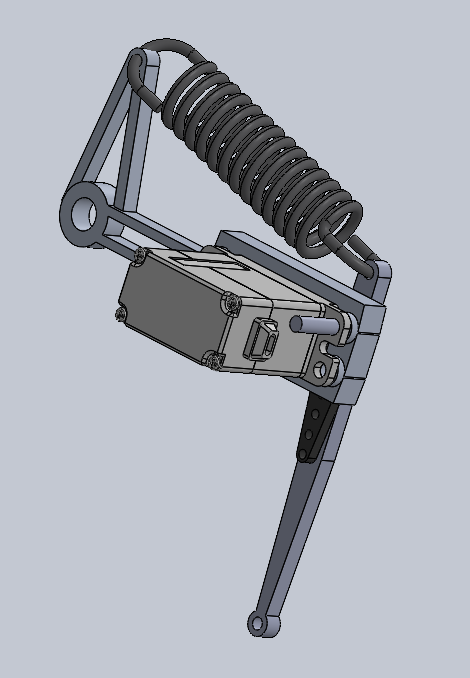
\includegraphics[width=\textwidth]{Images/extension_spring_outside.png}

        \label{fig:extension_spring_outside}
    \end{subfigure}
    \hfill
    \begin{subfigure}[b]{0.45\textwidth}
        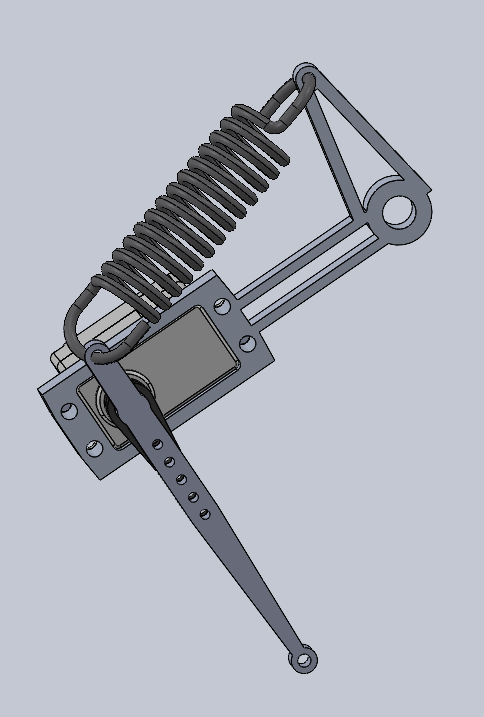
\includegraphics[width=\textwidth]{Images/extension_spring_inside.png}

        \label{fig:extension_spring_inside}
    \end{subfigure}
    \caption{Comparison of extension spring configurations: outside (left) and inside (right) the leg.}
    \label{fig:extension_spring_CAD}
\end{figure}

\subsection{Motor Selection}
\label{sec:motor_selection}

As discussed in section \ref{sec:robot_design}, the choice fell on AGF-RC motors due to their high torque to weight ratio, as well as our inability to find similarly fast motors of similar strength. 

Our specific choice of motors can be found in table \ref{tab:motor_selection}. Info about the specific motors can be found in appendices \ref{appendix:A06CLS_V2_website_information} to \ref{appendix:A20_info}.

\begin{table}[h!]
    \centering
    \begin{tabular}{|c|c|}
        \hline
        Corresponding Joint & Motor Name\\ \hline
        Knee flexion/extension & A20BHM \\
        Hip flexion/extension & A06CLS V2 \\
        Hip adduction/abduction & A06CLS V2 \\ \hline
    \end{tabular}
    \caption{Selected Motors}
    \label{tab:motor_selection}
\end{table}

The reason these motors in particular were chosen is the fact that no motors were found in a similar weight class that could provide the same torque and speed. For example, if considering AGF-RC motors, the next motor, strength-wise, after the A20BHM motor, is the A35CHM motor, info about which can be found in appendix \ref{appendix:A35CHM_motor_info}. Despite being significantly heavier, the A35CHM motor is only marginally stronger than the A20BHM motor. The reasoning behind the choice of the A06CLS V2 is detailed in section \ref{sec:hip_motor_dimensioning_test_design}.

It is worth mentioning that the mass of the thigh shown in figure \ref{fig:manufacture_only} is considerably higher than a similarly long thigh in the simulation, as described in section \ref{sec:modeling_and_simulation}. The main difference is that the thigh in the simulations is a long and thin rectangular prism, whereas the actual leg design is currently quite wide and bulky, so as to accommodate the motor and spring while maintaining structural integrity. This is a discrepancy between the simulations and the actual design, however, since the leg masses are so small compared to the mass of the motors and the main body, the discrepancy is not considered significant. For reference, the mass of the thigh for various material densities compared to the leg design used in simulation is shown in table \ref{tab:thigh_mass_comparison}.

\begin{table}[h!]
    \centering
    \begin{tabular}{|c|c|c|}
        \hline
        Material Density & Mass of thigh in simulation & Mass of actual thigh design \\ \hline
        1200 kg/m\textsuperscript{3} (Tough PLA, see appendix \ref{appendix:tough_PLA}) & N/A & 6.45 \\
        2700 kg/m\textsuperscript{3} (Aluminum 6061) & 2.26 g & 14.27 g \\
        \hline
    \end{tabular}
    \caption{Mass of thigh for various material densities compared to the leg design used in simulation. For the real thigh, mass properties were calculated using Solidworks "Mass Properties" tool. }
    \label{tab:thigh_mass_comparison}
\end{table}

\subsection{Other Purchased Components}

While the motors are the most important and expensive component constituting the leg, other components must also be purchased for its construction. A list of these components and their suppliers can be found in table \ref{tab:other_purchased_components}. Screws and nuts are not included. 

\begin{table}[h!]
    \centering
    \begin{tabular}{|c|c|c|}
        \hline
        Component & Name/Part Number & Supplier \\ \hline
        Bearing & RS: 612-5802 &  RS \\
        Left leg spring &  T075-180-484L & Sodemann\\
        Right leg spring &  T075-180-484R & Sodemann\\
        Knee servo horn & HPS06 & AGF-RC\\
        Hip servo horns & HPS065 & AGF-RC\\
        \hline
    \end{tabular}
    \caption{Other purchased components.}
    \label{tab:other_purchased_components}  
\end{table}